\begin{problem}[问题2.3]
考虑一个二维流场: $u=x(1+2t)$, $v=y$, $w=0$. 试确定并比较:
\begin{itemize}
\item [(a)] $t=0$时刻, 通过点$(1,1)$的流线;
\item [(b)] $t=0$时刻,通过点$(1,1)$的质点的迹线;
\item [(c)] 通过点$(1,1)$的质点在$t$时刻所形成的脉线.
\end{itemize}
\end{problem}
\begin{solution}
\begin{itemize}
\item [(a)]由流线微分方程:
\[
\frac{dx}{u} = \frac{dy}{v} \Longrightarrow \frac{dx}{x(1+2t)} = \frac{dy}{y}
\]
积分得流线方程
\[
\int \frac{dx}{x(1+2t)} = \int \frac{dy}{y} \Longrightarrow y = C x^{1/(1+2t)}
\]
其中$C$为常数.初始条件可得$C=1$, 故$t=0$时刻, 通过点$(1,1)$的流线为
\[
y = x
\]

\item [(b)]由迹线微分方程
\[
\frac{dx}{dt} = u = x(1+2t), {~}  \frac{dy}{dt} = v = y
\]
积分得
\[
x =  C_1 e^{t + t^2}, {~} y = C_2 e^t
\]
由初始条件得$C_1=C_2=1$, 故$t=0$时刻,通过点$(1,1)$的质点的迹线为
\[
x = e^{\ln y + (\ln y)^2}
\]

\item [(c)]由(b)中迹线参数方程
\begin{equation}\label{c}
x =  C_1e^{t + t^2}, {~} y = C_2e^t
\end{equation}
在$t_0$时刻时位置为$(1,1)$, 则有
\[
C_1 = \frac{1}{e^{t_0+t_0^2}}, {~} C_2 =\frac{1}{e^{t_0}}
\]
代入(\ref{c})式,得
\[
x =  \frac{1}{e^{t_0+t_0^2}} e^{t + t^2}, {~} y = \frac{1}{e^{t_0}}e^t
\]
清去$t_0$得通过点$(1,1)$的质点在$t$时刻所形成的脉线
\[
x = \frac{e^{t + t^2}}{e^{(t-\ln y)+(t - \ln y)^2}} = e^{(1+2t)\ln y - (\ln y)^2}
\]
\end{itemize}
\vspace{5pt}

\begin{multicols}{2} 
下面给出流线, 迹线, 脉线的定义及流线, 迹线, 脉线的曲线对比图(如图\ref{fig:StreamPathStreak}, 该图程序见附录\ref{sec:StreamPathStreak}). 对比发现, 对于本题, $t=0$时刻的迹线同时也是$t=0$时刻的脉线.
\begin{itemize}
\item \textbf{流线}是某一相同时刻在流场中画出的一条空间曲线, 在该时刻, 曲线上的所有质点的速度矢量均与这条曲线相切.
\item \textbf{迹线}是单个质点在连续时间过程内的流动轨迹线.
\item \textbf{脉线}是在某一时间间隔内相继经过空间一固定点的流体质点依次串连起来而成的曲线.
\end{itemize}
\begin{center}
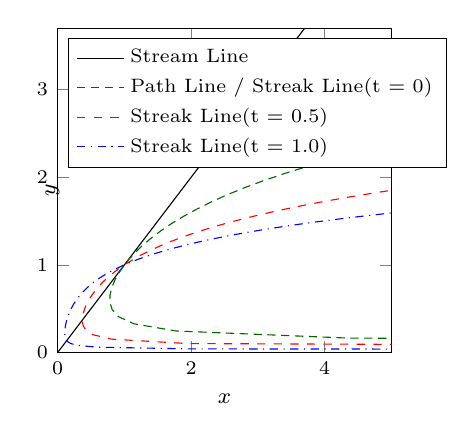
\begin{tikzpicture}
\begin{axis}[%
width=0.48\textwidth,
height=0.47\textwidth,
xmin=0,xmax=5,
xlabel={$x$},
ymin=0,ymax=3.7,
ylabel={$y$},
anchor=left of south west,
legend style={legend pos=north west,font=\scriptsize,legend cell align=left},
yticklabel style={font=\scriptsize},
xticklabel style={font=\scriptsize},
xlabel style={font=\footnotesize},
ylabel style={font=\footnotesize,yshift=-15pt},
]
\addplot [no markers,domain=0:4]{x};
\addlegendentry{Stream Line};

\addplot [no markers,densely dashed,domain=0:4,samples=50,green!40!black]({exp(ln(\x)+ln(\x)*ln(\x))},\x);
\addlegendentry{Path Line / Streak Line(t = 0)};

\addplot [no markers,dashed,domain=0:4,samples=80,red]({exp(2*ln(\x)+ln(\x)*ln(\x))},\x);
\addlegendentry{Streak Line(t = 0.5)};

\addplot [no markers,dashdotted,domain=0:4,samples=200,blue]({exp(3*ln(\x)+ln(\x)*ln(\x))},\x);
\addlegendentry{Streak Line(t = 1.0)};
\end{axis}
\end{tikzpicture}%

\captionof{figure}{流线, 迹线, 脉线的比较}\label{fig:StreamPathStreak}
\end{center}
\end{multicols}
\end{solution}
